\begin{figure*}[!t]
\centering
\subfloat[1]{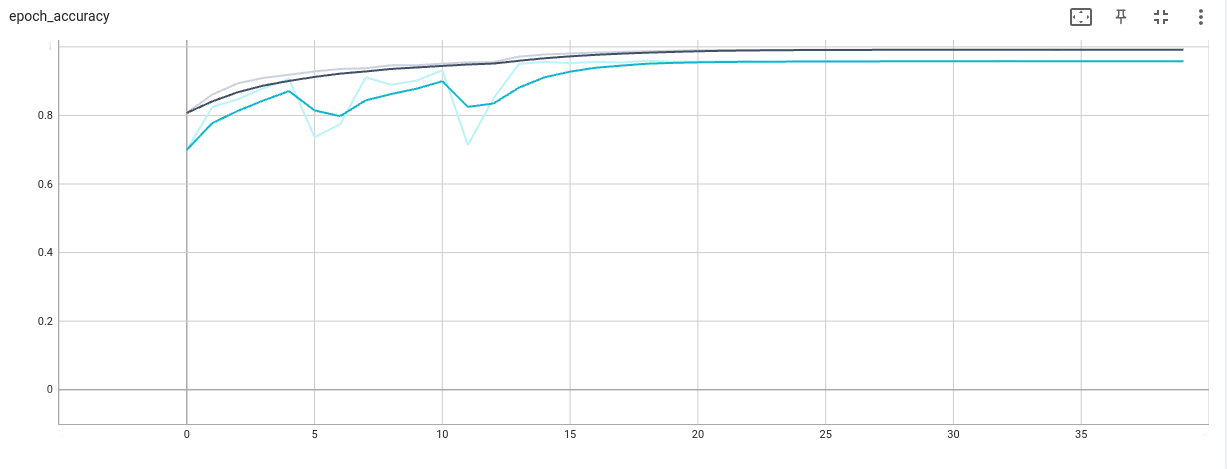
\includegraphics[angle=90, height=25cm, width=0.4\textwidth]{images/1_ac.png}}
\hfil
\subfloat[2]{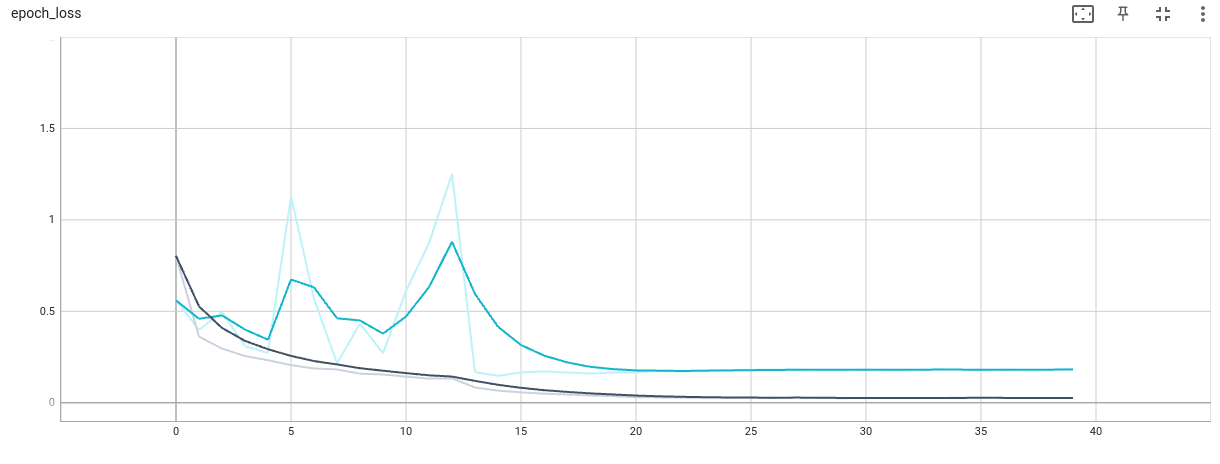
\includegraphics[angle=90, height=25cm, width=0.4\textwidth]{images/1_loss.png}
\caption{Model 1.}}
\label{model 1}
\end{figure*}

\begin{figure*}[!t]
\centering
\subfloat[1]{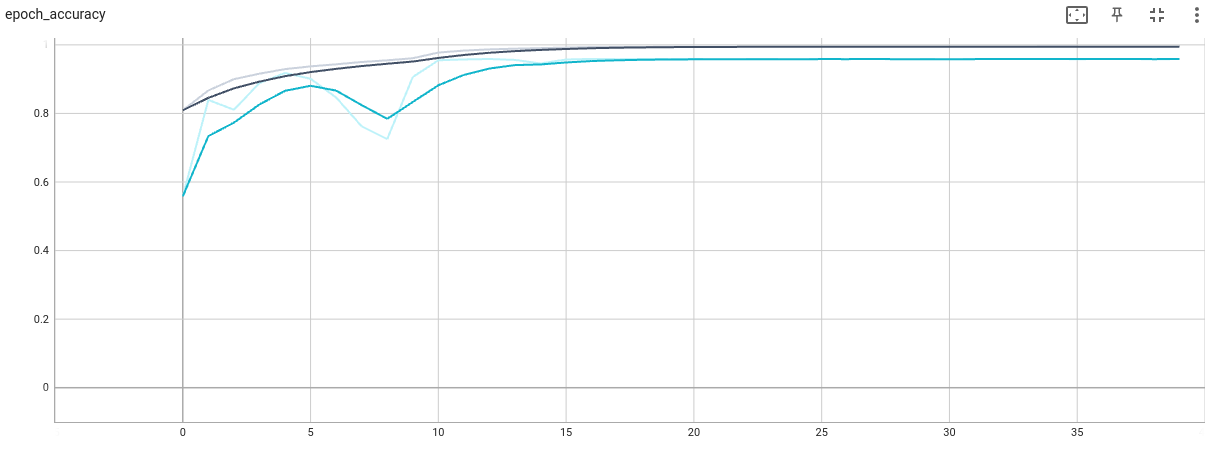
\includegraphics[angle=90, width=0.4\textwidth]{images/2_ac.png}}
\hfil
\subfloat[2]{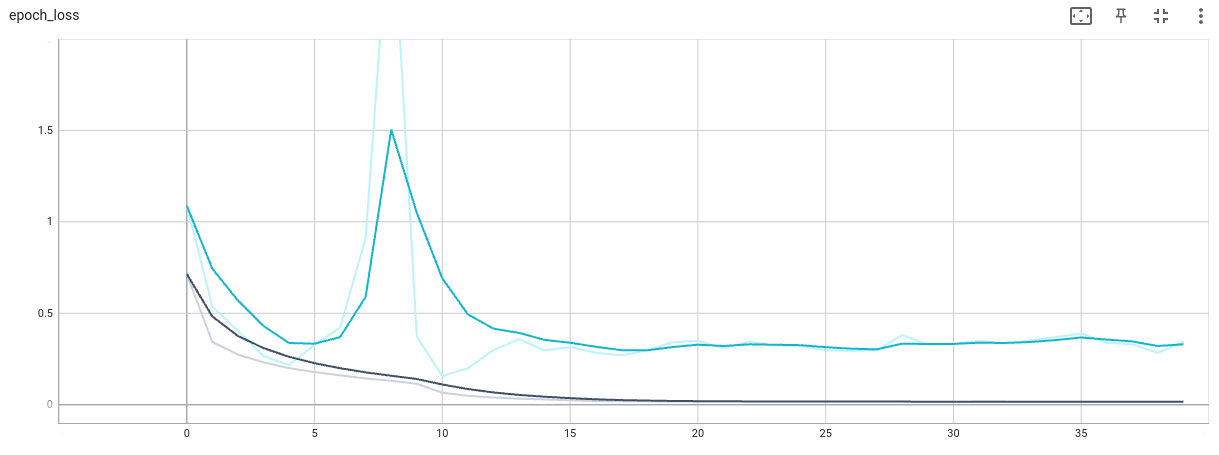
\includegraphics[angle=90, width=0.4\textwidth]{images/2_loss.png}
\caption{Model 2.}}
\label{model 2}
\end{figure*}

\begin{figure*}[!t]
\centering
\subfloat[1]{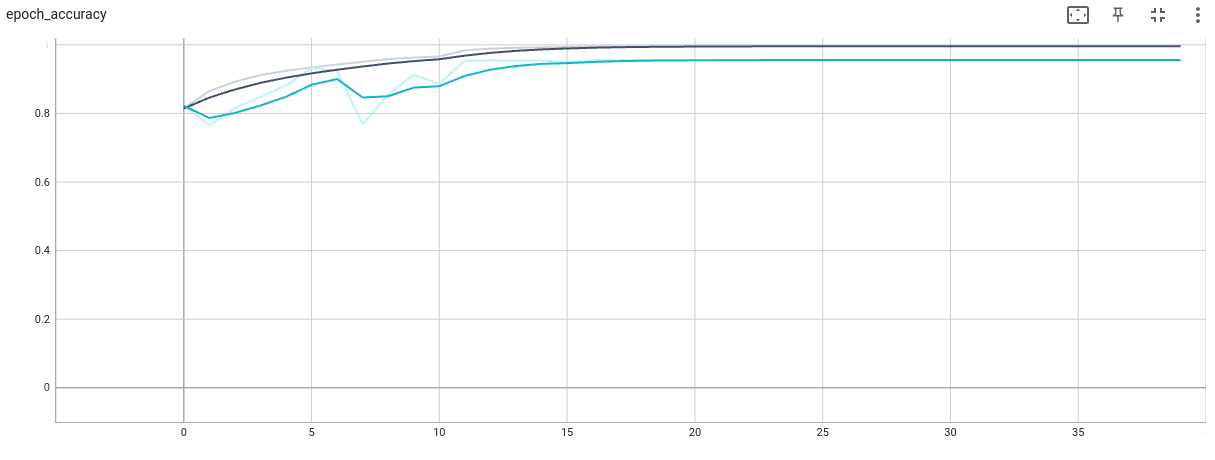
\includegraphics[angle=90, width=0.4\textwidth]{images/3_ac.png}}
\hfil
\subfloat[2]{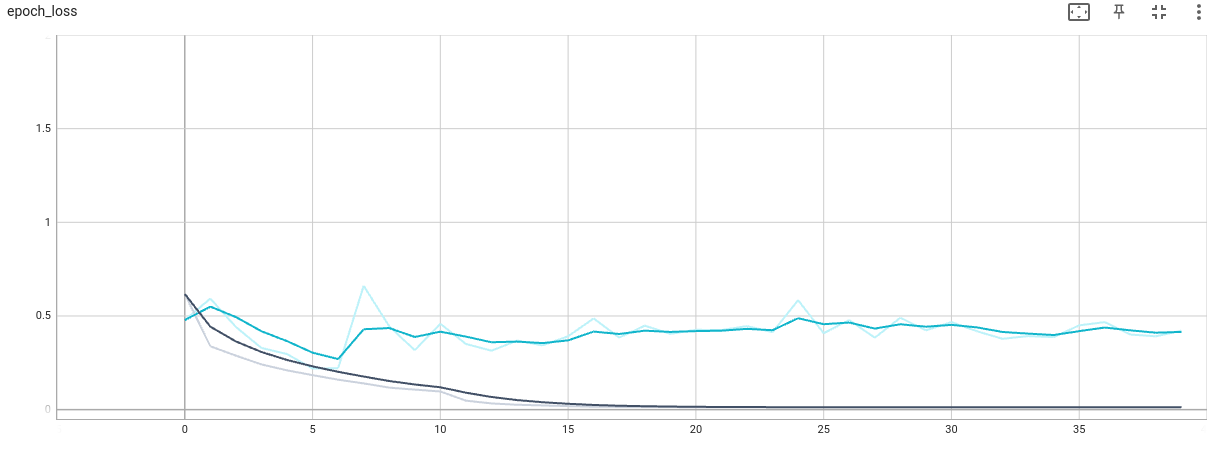
\includegraphics[angle=90, width=0.4\textwidth]{images/3_loss.png}
\caption{Model 3.}}
\label{model 3}
\end{figure*}

\begin{figure*}[!t]
\centering
\subfloat[1]{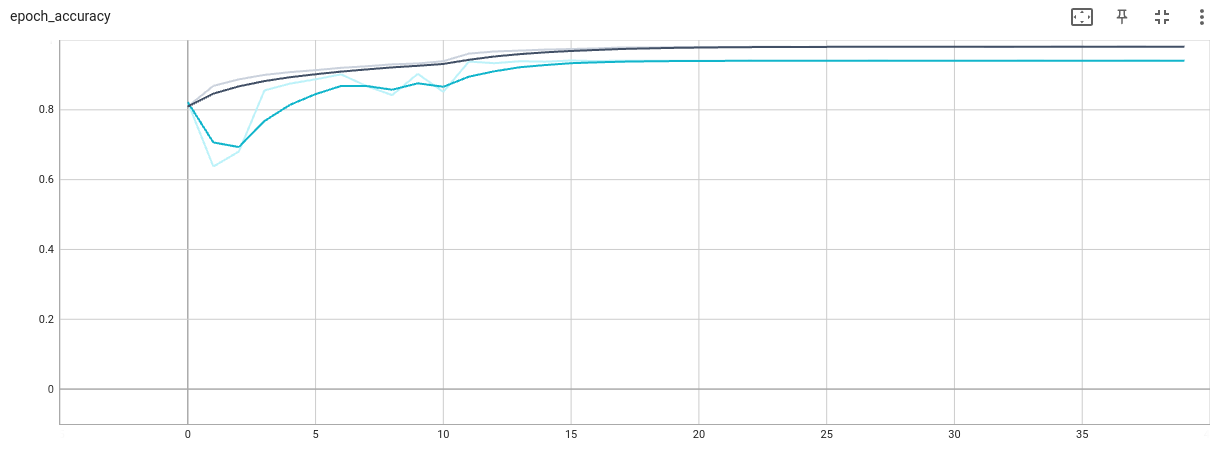
\includegraphics[angle=90, width=0.4\textwidth]{images/4_ac.png}}
\hfil
\subfloat[2]{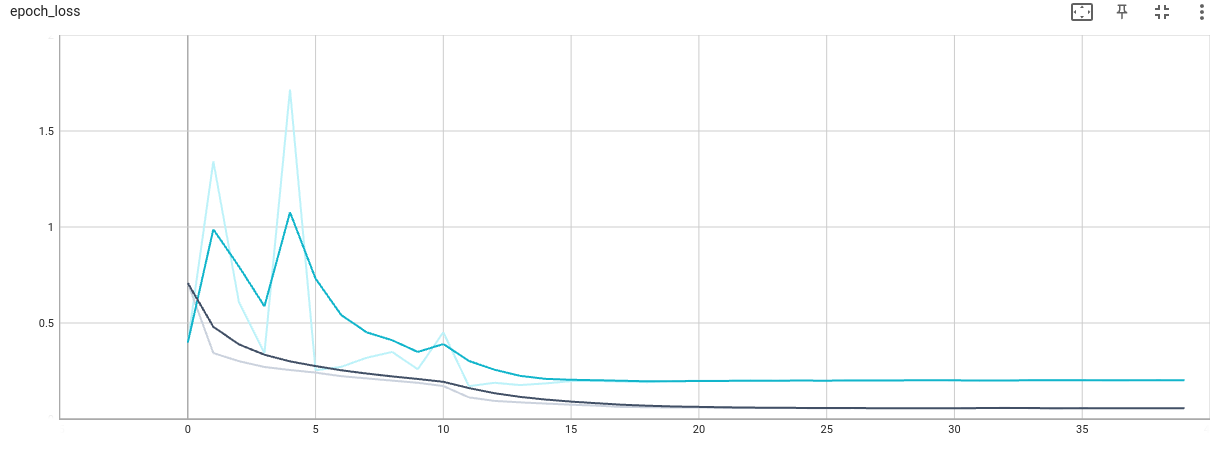
\includegraphics[angle=90, width=0.4\textwidth]{images/4_loss.png}
\caption{Model 4.}}
\label{model 4}
\end{figure*}

\begin{figure*}[!t]
\centering
\subfloat[1]{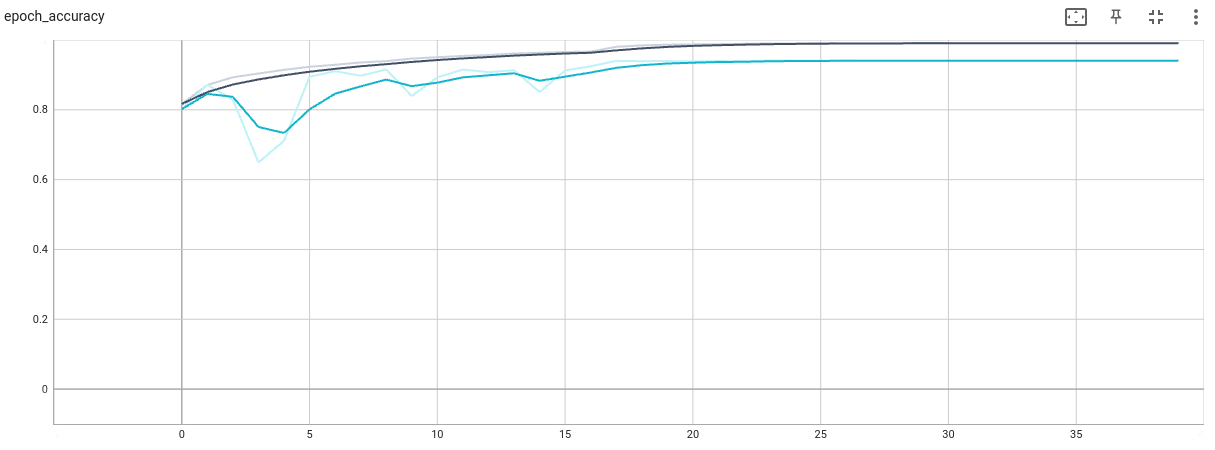
\includegraphics[angle=90, width=0.4\textwidth]{images/5_ac.png}}
\hfil
\subfloat[2]{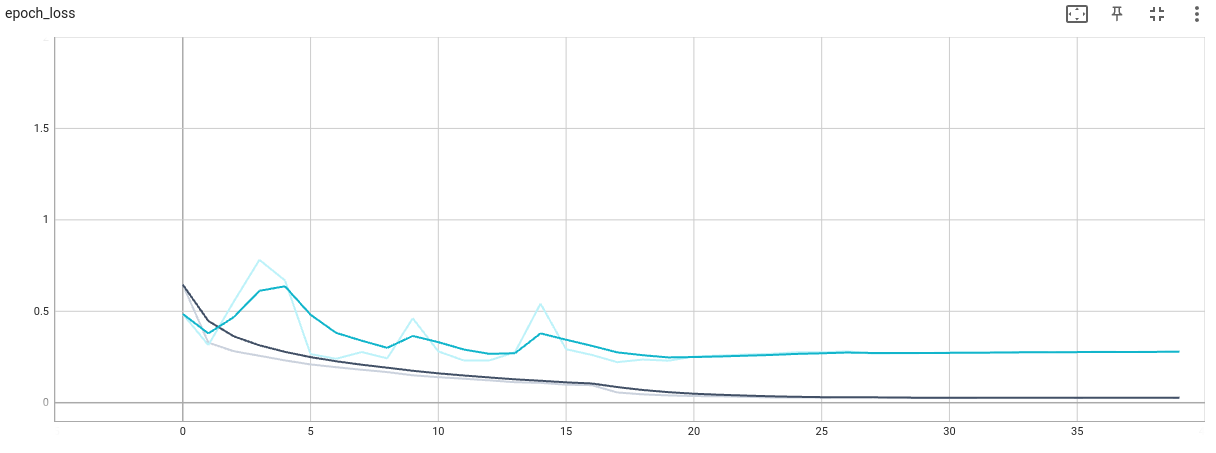
\includegraphics[angle=90, width=0.4\textwidth]{images/5_loss.png}
\caption{Model 5.}}
\label{model 5}
\end{figure*}

\begin{figure*}[!t]
\centering
\subfloat[1]{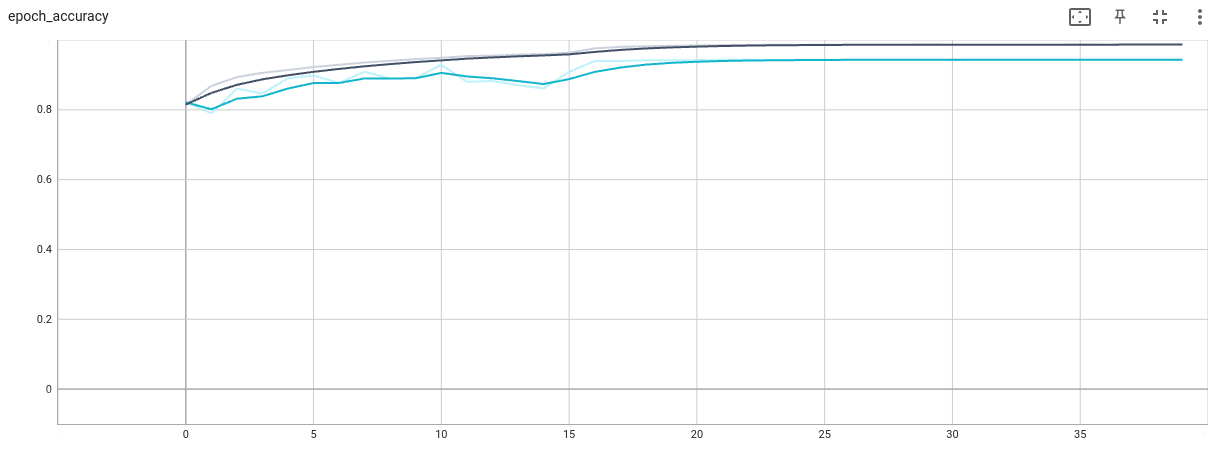
\includegraphics[angle=90, width=0.4\textwidth]{images/6_ac.png}}
\hfil
\subfloat[2]{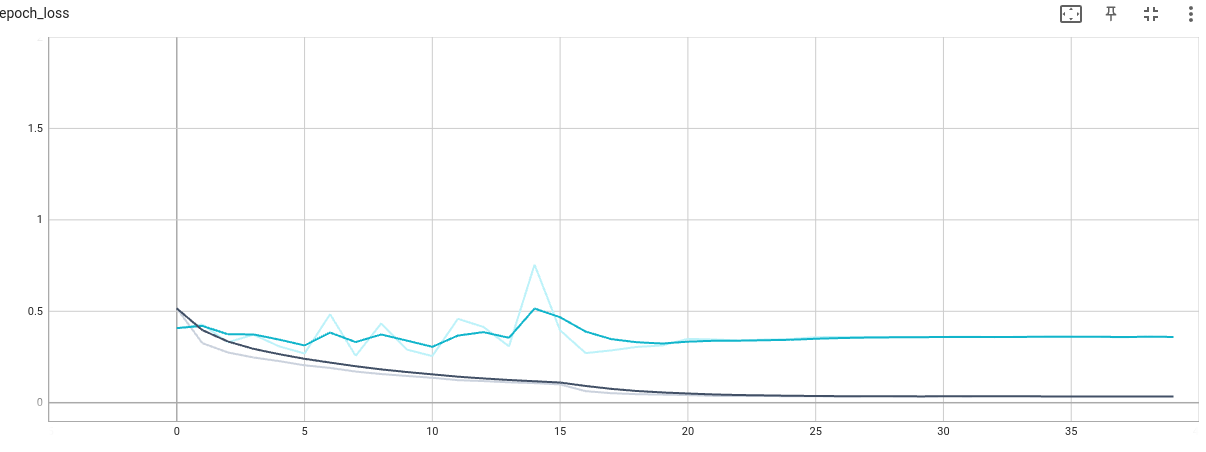
\includegraphics[angle=90, width=0.4\textwidth]{images/6_loss.png}
\caption{Model 6.}}
\label{model 6}
\end{figure*}

